%% ============================================================================
%%  x-map-reduce: IEEE Conference 论文
%%
%%  编译: make           (等价于 latexmk -pdf)
%%  预览: make view
%%  清理: make clean
%%
%%  写作约定:
%%    - 正文英文, 引用用 \cite{}
%%    - 图放 ../paper/bench/results/ 下, 由 results.mk 生成
%%    - 每个 TODO 注释标记待补内容, 完成后删除标记
%% ============================================================================
\documentclass[conference]{IEEEtran}
\IEEEoverridecommandlockouts

\usepackage{cite}
\usepackage{amsmath,amssymb,amsfonts}
\usepackage{algorithmic}
\usepackage{algorithm}
\usepackage{graphicx}
\usepackage{textcomp}
\usepackage{xcolor}
\usepackage{booktabs}      % 三线表
\usepackage{multirow}
\usepackage{url}
\usepackage{tikz}
\usepackage{pgfplots}
\pgfplotsset{compat=1.18}
\usetikzlibrary{arrows.meta,positioning,shapes,fit,backgrounds}

\def\BibTeX{{\rm B\kern-.05em{\sc i\kern-.025em b}\kern-.08em
    T\kern-.1667em\lower.7ex\hbox{E}\kern-.125emX}}

\begin{document}

\title{A Modern Re-implementation and Empirical Study of\\
MapReduce on Commodity Multiprocessors
\thanks{This work was completed as a course project.}}

\author{
\IEEEauthorblockN{Rui Ding}
\IEEEauthorblockA{\textit{Software Engineering Institute}\\
\textit{East China Normal University}\\
Shanghai, China\\
71295902014@stu.ecnu.edu.cn}
\and
\IEEEauthorblockN{Beibei Huang}
\IEEEauthorblockA{\textit{Software Engineering Institute}\\
\textit{East China Normal University}\\
Shanghai, China\\
71295902023@stu.ecnu.edu.cn}
\and
\IEEEauthorblockN{Kairui Li}
\IEEEauthorblockA{\textit{Software Engineering Institute}\\
\textit{East China Normal University}\\
Shanghai, China\\
71295902039@stu.ecnu.edu.cn}
\and
\IEEEauthorblockN{Wenkai Wang}
\IEEEauthorblockA{\textit{Software Engineering Institute}\\
\textit{East China Normal University}\\
Shanghai, China\\
71295902070@stu.ecnu.edu.cn}
}

\maketitle

%% ===========================================================================
\begin{abstract}
MapReduce~\cite{dean2004mapreduce} remains a canonical model for large-scale
data processing, yet its original implementation was tied to a specific
cluster environment and is largely opaque today. We present
\textbf{x-map-reduce}, a from-scratch C++20 re-implementation of the
MapReduce programming model that runs on commodity hardware, and report an
empirical study of its behaviour. Our design separates a control plane for
metadata from a data plane for bulk transfer, delegates shuffle to
worker-to-worker partitions, ships job logic as content-addressed native
plugins, and layers a GFS-style block store underneath.
Scaling experiments on a single eight-core machine show that increasing the
worker count from one to six reduces word-count job time by only
$1.55\times$ on a 10\,MB input and $1.46\times$ on a 20\,MB input, far from
the ideal $6\times$; on the larger input, going from four to six workers
actually makes the job slower.
Profiling attributes the gap to two serial stages inside each reduce task---a
sequential fetch of all map outputs and a sort-then-tree-insert grouping
step---which bound throughput independently of the number of workers. We
quantify the effect of reduce-partition count, which acts as the effective
parallelism knob, and discuss what these results imply for small-scale
MapReduce deployments.
\end{abstract}

\begin{IEEEkeywords}
MapReduce, distributed systems, fault tolerance, performance evaluation,
plugin architecture
\end{IEEEkeywords}

%% ===========================================================================
\section{Introduction}
\IEEEPARstart{M}{apReduce}, introduced by Dean and Ghemawat~\cite{dean2004mapreduce},
provides a simple abstraction for processing large datasets: users supply a
\textit{map} function and a \textit{reduce} function, and the runtime handles
parallelisation, data distribution, and fault recovery.

The model was formulated for a specific environment: hundreds of commodity
machines in a single datacenter, each with one or two cores, a local disk,
and a shared network. Many of its design choices follow from that setting.
Computation is pushed to the data because moving bytes across the network
was the expensive operation. The coordinator is centralised because the
cluster was large enough that the resulting single point of contention was
tolerable. Tasks are short and are simply re-run on failure because a
recomputation over a local disk is cheap.

Modern hardware violates several of these premises. A single multi-core
machine today has more compute than an entire cluster from 2004, with
orders of magnitude more memory bandwidth and no network between cores.
It is therefore worth asking which parts of the original design still
pay off, and which have become the bottleneck. Answering that question
requires a system we can instrument, measure, and modify---which existing
production implementations, optimised over more than a decade for
scale-out deployments, are not well suited to.

This paper reports on x-map-reduce, a from-scratch re-implementation of
the MapReduce model in C++20 targeted at commodity multiprocessors, and on
what happens when it is measured. We did not set out to build a faster
MapReduce; we set out to understand one.

The headline result is negative and, we think, instructive. Adding workers
helps far less than the model suggests: six workers complete a 10\,MB
word-count job only $1.55\times$ faster than one, and on a 20\,MB input the
sixth pair of workers makes the job measurably slower than four. The reason
is not scheduling overhead but two serial stages inside each reduce task,
which bound overall throughput independently of how many workers are
available.
A second finding concerns fault tolerance: a fixed task timeout, calibrated
for small inputs, misclassified genuine progress as failure at larger
sizes, and the resulting error message named the wrong component. Both
findings are properties of the design, not of our implementation effort.

The contributions of this paper are:
\begin{itemize}
    \item \textbf{A complete re-implementation.} We describe
          x-map-reduce, an approximately 10k-line C++20 implementation
          covering scheduling, shuffle, block storage, and fault handling
          (Sec.~\ref{sec:design}, Sec.~\ref{sec:impl}).
    \item \textbf{A design that separates control and data planes} and
          moves shuffle off the coordinator, together with a
          content-addressed plugin mechanism for job submission
          (Sec.~\ref{sec:design}).
    \item \textbf{An empirical characterisation} of its behaviour on
          commodity hardware, including scalability, the dominant role of
          reduce-partition count, and recovery under worker failure
          (Sec.~\ref{sec:eval}), together with the lessons those
          measurements suggest (Sec.~\ref{sec:lessons}).
\end{itemize}

%% ===========================================================================
\section{Related Work}
\label{sec:related}

%% TODO: 必写. 建议覆盖:
%%   1. 原始 MapReduce / GFS
%%   2. Hadoop, Spark, Dryad, FlumeJava (数据流抽象演进)
%%   3. 推测执行 (LATE, Mantri)
%%   4. 现代硬件下 MapReduce 仍相关的讨论

\textbf{MapReduce and GFS.} The original system~\cite{dean2004mapreduce}
and its storage substrate~\cite{ghemawat2003gfs} established the model of
computation moved to data, with redundant placement and re-execution as the
primary fault-tolerance mechanism.

\textbf{Dataflow successors.} Dryad~\cite{isard2007dryad},
Spark~\cite{zaharia2012spark}, and FlumeJava~\cite{chambers2010flumejava}
generalise the two-stage map/shuffle/reduce pipeline to arbitrary dataflow
graphs, primarily to avoid materialising intermediate results.

%% TODO: Hadoop 引用请补正式出处
\textbf{Open-source implementations.} Hadoop MapReduce has served as the
de-facto reference implementation for over a decade, fixing many of the
operational details the original paper leaves implicit---container-based
execution, a centralised resource negotiator, and on-disk shuffle.

\textbf{Speculative execution.} The original system guards against stragglers
by launching backup tasks near the end of a job. Later work refines the
trigger: LATE~\cite{zaharia2008late} estimates remaining time from progress
rates rather than using a fixed threshold, and Mantri~\cite{ananthanarayanan2010mantri}
attributes stragglers to causes such as network congestion and re-runs work
accordingly. Our implementation uses a static threshold, which
Sec.~\ref{sec:lessons} identifies as a limitation.

\textbf{Positioning.} Our work does not propose a new execution model.
It revisits the classic design on hardware that did not exist when the model
was defined---commodity multi-core machines rather than racks of single-core
disks---and reports where the original design decisions stop paying off.

%% ===========================================================================
\section{System Design}
\label{sec:design}

\subsection{Overview}

x-map-reduce consists of three roles: a persistent coordinator
(\texttt{x-master}), persistent workers (\texttt{x-worker}), and a client
(\texttt{xmr-submit}). Fig.~\ref{fig:arch} shows the deployment.

Unlike the original design, in which a single master process is created per
job and exits when the job finishes, both the coordinator and the workers are
long-lived processes. The coordinator serves one job at a time through a
per-job \emph{coordinator} object that is created on submission, drives the
job to completion, and then resets; the process itself keeps running and
keeps its worker connections and heartbeats alive. This avoids paying
connection setup and worker registration costs on every submission, and it
makes the failure-detection machinery meaningful---a watchdog is only useful
if the things it watches persist across jobs.

A job proceeds in four phases. On submission the client uploads the plugin
and provides DFS paths; the coordinator resolves each path to its blocks and
creates one map task per block. Map tasks execute on the workers holding the
relevant blocks, each partitioning its output into $R$ files, one per reduce
partition. Reduce tasks then fetch their partition from every map task's host
and group by key. Finally the coordinator streams results back to the
client and releases the job's blocks.

\begin{figure}[t]
\centering
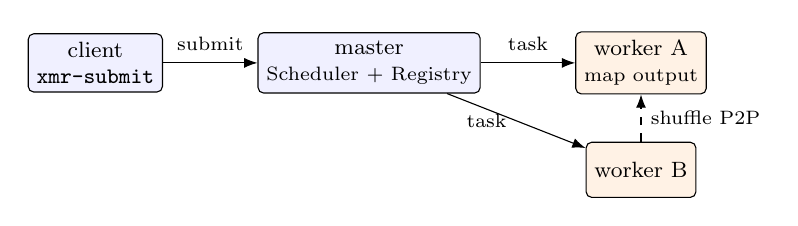
\begin{tikzpicture}[
    font=\footnotesize,
    node distance=4mm,
    box/.style={draw, rounded corners=2pt, align=center, inner sep=3pt, minimum height=7mm},
    ent/.style={box, fill=blue!6},
    dat/.style={box, fill=orange!10}
]
  \node[ent] (c) {client\\\texttt{xmr-submit}};
  \node[ent, right=12mm of c] (m) {master\\\scriptsize Scheduler + Registry};
  \node[dat, right=12mm of m] (w1) {worker A\\\scriptsize map output};
  \node[dat, below=6mm of w1] (w2) {worker B};
  \draw[-{Latex}] (c) -- node[above,yshift=1pt]{\scriptsize submit} (m);
  \draw[-{Latex}] (m) -- node[above,yshift=1pt]{\scriptsize task} (w1);
  \draw[-{Latex}] (m) -- node[left]{\scriptsize task} (w2);
  \draw[-{Latex}, dashed] (w2) -- node[right]{\scriptsize shuffle P2P} (w1);
\end{tikzpicture}
\caption{Deployment and control/data plane separation.}
\label{fig:arch}
\end{figure}

\subsection{Control Plane and Data Plane}

The coordinator handles only metadata: submission, worker registration,
heartbeats, and task assignment. Bulk data never traverses it. Map outputs
stay on the worker that produced them, and the coordinator records only the
mapping from map task to host so that reducers know where to fetch. This
keeps coordinator message volume a function of task count rather than data
size, and it lets the coordinator remain a simple single-threaded reactor.

A consequence is that losing a worker invalidates its map outputs, not just
its tasks. The coordinator therefore has to re-run completed map tasks whose
output no longer exists, which we handle by treating such maps as
unfinished.

\subsection{Worker to Worker Shuffle}

Map output is partitioned at the map side using a hash of the key modulo the
number of reduce partitions, so each reducer reads one partition per map
task directly from the producing worker's data listener. With $M$ map tasks
and $R$ reduce partitions the transfer graph is $M \times R$ independent
point-to-point streams rather than $2M$ streams funnelled through the
coordinator.

\subsection{Content-Addressed Plugins}

Job logic ships as a native shared object rather than as code compiled into
the workers. Plugins are named by content hash, cached on each worker, and
loaded through \texttt{dlopen}; the ABI is a versioned
\texttt{extern "C"} entry point returning a job descriptor. Because the
identity of a plugin is its hash, workers can cache aggressively and the
coordinator never needs to reason about version skew.

\subsection{Block Storage and Locality}

Input is stored as fixed-size 1\,MiB blocks with replicas placed across
workers. One block becomes one map task by default, so the number of map
tasks is determined by input size. The coordinator prefers to assign a map
task to a worker that already holds the block, falling back to any idle
worker when no replica is free, which yields data locality without a
separate scheduler.

\subsection{Design Trade-offs}

Three of these decisions carry costs that only became visible once the
system was measured, and we state them explicitly rather than presenting the
design as unproblematic.

\textbf{Peer-to-peer shuffle is not free.} Keeping bulk data off the
coordinator makes the coordinator scale, but it makes each reducer
responsible for gathering its own input. Because one block is one map task,
a reducer must contact as many peers as there are blocks. Making the block
size smaller improves parallelism but increases this fan-in; making it
larger reduces fan-in but coarsens scheduling. Our 1\,MiB choice, inherited
from the block-storage layer, is a compromise that we did not tune, and
Sec.~\ref{sec:eval} shows the consequence.

\textbf{Content addressing assumes compatible machines.} Shipping native
code works because every worker runs the same binary interface on the same
architecture. Across heterogeneous hardware a plugin cache keyed by content
hash would be incorrect, and the mechanism would have to fall back to
source distribution or bytecode. This is an acceptable assumption for a
single-machine deployment and a poor one for a mixed cluster.

\textbf{A centralised coordinator remains a single point of failure.}
Replicating it requires persistent job state, which the current
implementation does not keep; recovering a coordinator after restart would
therefore lose in-flight jobs even though worker data survives. Our fault
experiments consequently cover worker loss only.

%% ===========================================================================
\section{Implementation}
\label{sec:impl}

The implementation is approximately 10\,000 lines of C++20. Table~\ref{tab:loc}
gives the per-module breakdown.

\begin{table}[t]
\caption{Implementation size by module (lines of C++)}
\label{tab:loc}
\centering
\begin{tabular}{@{}lr@{}}
\toprule
Module & Lines \\
\midrule
protocol & 2\,162 \\
tests & 1\,904 \\
master & 1\,836 \\
dfs & 1\,208 \\
runtime & 1\,098 \\
worker & 950 \\
client & 658 \\
mapreduce & 334 \\
server & 265 \\
jobs & 69 \\
\midrule
total & 10\,484 \\
\bottomrule
\end{tabular}
\end{table}

\subsection{Event-Driven Runtime}

Each process runs an epoll-based reactor. Network I/O is handled by a small
number of I/O threads, while task execution---map and reduce functions---is
offloaded to a worker thread pool so that a long computation never blocks the
event loop. The coordinator runs a fixed-interval tick, modelled on Pregel's
super-steps, that drives scheduling, heartbeat expiry, and task timeouts.

\subsection{Wire Protocol}

All control messages share one binary framing: a 16-byte big-endian header
carrying magic (\texttt{XMRP}), version, type, flags, a request identifier,
and a payload length capped at 64\,MiB, followed by a variable-length body.
Strings and blobs are length-prefixed rather than delimiter-separated, so the
codec is binary-safe. Framing is the only thing the transport layer knows;
message semantics live in a separate module, and version mismatch is resolved
by a \textsc{hello}/\textsc{hello\_ack} exchange before any other message is
accepted.

\subsection{Fault Tolerance Mechanisms}

Three mechanisms operate together. A heartbeat watchdog marks a worker lost
after $6$\,s of silence and requeues whatever it held. A per-task watchdog
re-dispatches a task that has not reported completion within $30$\,s, even if
its worker is still alive. Speculative execution duplicates a task when it
has run longer than $\max(3\,\text{s}, 2\times\text{fastest completed
attempt})$ and a spare worker is idle; the first attempt to finish wins and
the loser is cancelled.

Retries are idempotent by construction: each attempt carries an identifier,
and a late result from a superseded attempt is discarded rather than allowed
to overwrite the current one. After four attempts a task is declared failed
and the job aborts. As Sec.~\ref{sec:eval} shows, this fixed timeout is the
component most sensitive to workload scale.

%% ===========================================================================
\section{Evaluation}
\label{sec:eval}

\subsection{Experimental Setup}

All experiments run on a single machine with an 8-core Intel Xeon Platinum
8272CL (2.60\,GHz, one thread per core) and 7.5\,GB of RAM running
CentOS Stream 9. The coordinator and all workers are separate processes on
this machine communicating over the loopback interface; we cap concurrency
at six workers to leave headroom for co-resident services.

The workload is word count over synthetic text. Input is generated to a
fixed byte size with a vocabulary of 2\,000 distinct tokens and five tokens
per line. Because the input is partitioned into 1\,MiB blocks and each block
becomes one map task, a 10\,MB job comprises ten map tasks. Input files are
ingested into the block store before each measurement, and job duration is
measured from submission until the coordinator acknowledges the result, so
it includes scheduling, mapping, shuffle, and reduce. Each configuration is
measured three times; we report the median.

\subsection{Scalability}

Fig.~\ref{fig:scaling} plots job duration against worker count for 10\,MB
and 20\,MB inputs, and Table~\ref{tab:scaling} gives the medians of three
runs per configuration.

\begin{table}[t]
\caption{Job duration (median of 3 runs) and speed-up relative to one worker}
\label{tab:scaling}
\centering
\begin{tabular}{@{}rcccc@{}}
\toprule
 & \multicolumn{2}{c}{10\,MB} & \multicolumn{2}{c}{20\,MB} \\
\cmidrule(lr){2-3}\cmidrule(lr){4-5}
Workers & s & Speed-up & s & Speed-up \\
\midrule
1 & 18.67 & 1.00$\times$ & 37.86 & 1.00$\times$ \\
2 & 15.53 & 1.20$\times$ & 28.58 & 1.32$\times$ \\
4 & 13.03 & 1.43$\times$ & 25.48 & 1.49$\times$ \\
6 & 12.01 & 1.55$\times$ & 25.88 & 1.46$\times$ \\
\midrule
ideal & & $W\times$ & & $W\times$ \\
\bottomrule
\end{tabular}
\end{table}

\begin{figure}[t]
\centering
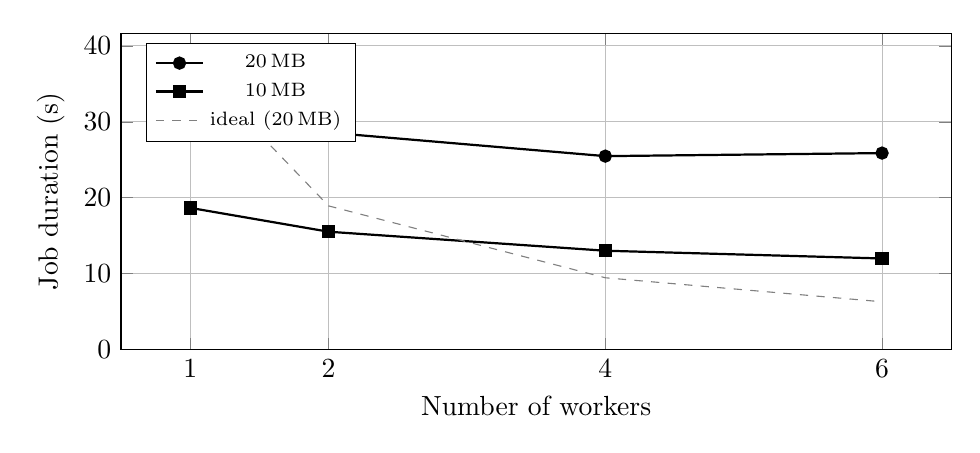
\begin{tikzpicture}
\begin{axis}[
    width=\columnwidth, height=5.6cm,
    xlabel={Number of workers}, ylabel={Job duration (s)},
    xtick={1,2,4,6}, ymin=0, xmin=0.5, xmax=6.5,
    legend pos=north west,
    legend style={font=\scriptsize},
    grid=major
]
\addplot[mark=*, thick] coordinates {(1,37.86) (2,28.58) (4,25.48) (6,25.88)};
\addlegendentry{20\,MB}
\addplot[mark=square*, thick] coordinates {(1,18.67) (2,15.53) (4,13.03) (6,12.01)};
\addlegendentry{10\,MB}
\addplot[mark=none, dashed, gray] coordinates {(1,37.86) (2,18.93) (4,9.47) (6,6.31)};
\addlegendentry{ideal (20\,MB)}
\end{axis}
\end{tikzpicture}
\caption{Job duration versus worker count. Both curves flatten well before
the available core count, and the larger input turns upward at six workers.}
\label{fig:scaling}
\end{figure}

Adding workers yields strongly diminishing returns on both inputs. For
10\,MB the first extra worker buys $1.20\times$, but the last two workers
together add only $8\%$; total duration falls from 18.67\,s to 12.01\,s over
a six-fold increase in workers, a speed-up of $1.55\times$.

The 20\,MB curve is more informative. It tracks closer to linear up to four
workers ($1.49\times$) and then \emph{regresses}: six workers take 25.88\,s
against 25.48\,s at four. The job gets slightly slower when given more
resources. This is the signature of a bottleneck that is not shared and
therefore cannot be amortised: past four workers, additional workers add
contention and scheduling overhead without shortening the critical path.

\subsection{Methodology and Threats to Validity}

Before interpreting the curve we address factors that could produce it
artificially, since a flat scaling curve is easy to obtain for the wrong
reasons.

\textbf{Co-resident services.} The machine also runs unrelated containerised
services. We cap the worker count at six on eight cores and leave the rest
for those services. This means absolute timings are slightly pessimistic,
but it does not explain the \emph{shape} of the curve: with six workers and
two spare cores, neither core oversubscription nor memory exhaustion
occurred in these runs.

\textbf{Measurements include fixed costs.} Job duration is measured from
submission to result acknowledgement, so it includes process start-up,
worker registration, and plugin distribution. These are per-job rather than
per-worker costs, and they inflate all points roughly equally---which if
anything would flatten the curve. To check, we measured a 10\,MB input
ingestion alone at $1.6$--$2.4$\,s, a small fraction of the $12$--$20$\,s
job time, confirming that fixed I/O overhead is not dominant.

\textbf{Run-to-run variance.} Each configuration is measured three times.
Observed spread is within about $10\%$ of the median, well below the
differences between configurations, so the ordering of the medians is
stable across repetitions.

\textbf{Single host.} All workers share one machine and communicate over
loopback. This removes network cost from the shuffle entirely, and is
therefore the \emph{most favourable} setting for scaling in which shuffle
is the constraint. Any bottleneck we observe here can only be worse when
workers are spread across physical hosts. Conversely, the experiment cannot
speak to network effects, which is a limitation we return to in
Sec.~\ref{sec:lessons}.

\subsection{Why Scaling Stalls: The Reduce Bottleneck}

The flat curve is not a scheduling artefact. Profiling the implementation
identifies two serial stages that bound overall throughput regardless of how
many workers are available.

First, a reduce task fetches the output of \emph{every} map task into a
single in-memory vector before it begins reducing
(\texttt{runtime/src/task.cpp}). The number of map tasks grows linearly with
input size, so the per-reducer working set grows with the job, and this
fetch loop is sequential.

Second, grouping sorts the entire intermediate dataset and then inserts
every element into an ordered map
(\texttt{mapreduce/src/mapreduce.cpp}). The sort already establishes key
order, yet an additional tree insertion per element follows, making this
stage $O(n \log n)$ with a large constant.

Both stages execute inside a single reduce task, so they do not overlap
across workers. Consequently overall time is dominated by the slowest
reducer rather than by the aggregate map throughput.

\subsection{Effect of Reduce Partitions}

%% TODO: 待补: reducers 单独扫描实验(固定 worker 数, 变化 reducers)

Since the reduce stage is serial per task, the number of reduce partitions
\emph{is} the parallelism knob. In a preliminary sweep over a 10\,MB input
with four workers, durations were 19.21\,s, 12.28\,s, and 13.04\,s for one,
four, and eight reducers respectively (Fig.~\ref{fig:reducers}). Moving from
one to four partitions cuts duration by roughly a third, while increasing
further to eight yields no benefit---consistent with the available worker
count, beyond which extra partitions only add overhead.

\begin{figure}[t]
\centering
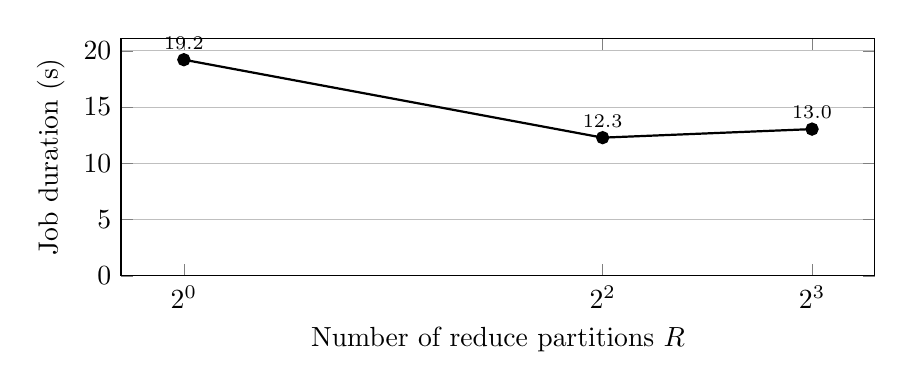
\begin{tikzpicture}
\begin{axis}[
    width=0.92\columnwidth, height=4.6cm,
    xlabel={Number of reduce partitions $R$},
    ylabel={Job duration (s)},
    xtick={1,4,8}, xmode=log, log basis x=2,
    ymajorgrids, ymin=0,
    nodes near coords, point meta=y,
    nodes near coords style={font=\scriptsize, /pgf/number format/.cd,
                             fixed, fixed zerofill, precision=1},
]
\addplot[mark=*, thick] coordinates {(1,19.21) (4,12.28) (8,13.04)};
\end{axis}
\end{tikzpicture}
\caption{Effect of reduce-partition count at four workers, 10\,MB input.
Four partitions is the sweet spot; beyond it, duration increases again.}
\label{fig:reducers}
\end{figure}

The shape is explained by the two competing effects. Too few partitions
concentrates all intermediate data into a single serial reduce task. Too
many partitions creates more tasks than there are workers, so partitions
queue behind one another while each still pays the fixed cost of fetching
from all map tasks. The optimum therefore tracks the worker count rather
than the data size---which is itself a symptom of the underlying problem,
because a well-partitioned shuffle need not care how many workers run the
reduce phase.

\subsection{Interaction Between Memory Pressure and Task Timeouts}

A second, less expected failure mode appeared at larger input sizes and is
worth reporting because its diagnosis is counter-intuitive.

On a 50\,MB input with four workers, jobs failed consistently, always after
roughly $30$\,seconds, with the error \texttt{map task 0 failed: attempts
exhausted}. Two observations seemed contradictory. First, an isolated 1\,MiB
map task completes in about $1.26$\,s, far below any plausible timeout.
Second, sampling resident memory during the run shows aggregate worker RSS
climbing monotonically from $0.2$\,GB at $2$\,s to $2.65$\,GB at $30$\,s
before falling back:

\begin{center}
\begin{tabular}{@{}rrrrrr@{}}
\toprule
$t$ (s) & 2 & 10 & 20 & 30 & 34 \\
\midrule
RSS (GB) & 0.22 & 0.72 & 1.34 & 2.65 & 0.96 \\
\bottomrule
\end{tabular}
\end{center}

The memory growth originates in reduce, not map: each reduce task pulls the
output of all fifty map tasks into memory at once before sorting. Under this
pressure the worker's event loop slows, map tasks overrun the coordinator's
hard-coded $30$\,s \texttt{kTaskTimeout}, and the coordinator re-dispatches
them. After four attempts (\texttt{maxAttempts}~$=4$) the job is declared
failed. The reported error blames map task~0, but the root cause lies
entirely in the reduce path.

To confirm, we raised \texttt{kTaskTimeout} from $30$\,s to $600$\,s,
recompiled, and re-ran the identical 50\,MB job. It completed successfully
in $56.3$\,s with correct output (2\,000 distinct keys). The system was
always capable of the work; the timeout policy, calibrated for small inputs,
was misclassifying progress as failure. Increasing the number of reduce
partitions did \emph{not} help---the job still failed at $30.1$\,s with
sixteen partitions---because partition count does not reduce the total
intermediate data each worker must buffer.

\subsection{Fault Recovery}

We inject a fault by killing one worker with \texttt{SIGKILL} at a fixed
delay after job submission, leaving three of the four workers alive, and
measure whether the job still completes. Table~\ref{tab:fault} reports the
results over a 10\,MB input; the fault-free baseline for the same
configuration is $12.46$--$13.42$\,s.

\begin{table}[t]
\caption{Fault recovery: one worker killed mid-job (4 workers, 10\,MB)}
\label{tab:fault}
\centering
\begin{tabular}{@{}cccc@{}}
\toprule
Kill after & Duration (s) & Recovered & Output keys \\
\midrule
1\,s & 12.42 & \checkmark & 2\,000 \\
2\,s & 12.57 & \checkmark & 2\,000 \\
3\,s & 13.29 & \checkmark & 2\,000 \\
\bottomrule
\end{tabular}
\end{table}

All three runs completed with correct output, and the overhead relative to
the fault-free baseline is negligible ($0.0\%$, $0.9\%$, and $6.6\%$).
The recovery path is therefore cheap at this scale: the coordinator detects
the loss through the heartbeat mechanism, re-dispatches the affected tasks
to surviving workers, and the job proceeds. The later the fault is injected,
the more work has already completed, so the marginal cost grows slightly.

We note that this experiment exercises worker loss, not coordinator loss.
The coordinator remains a single point of failure in the current
implementation, as discussed in Sec.~\ref{sec:lessons}.

%% ===========================================================================
\section{Lessons Learned}
\label{sec:lessons}

Building and measuring the system surfaced several observations that we
believe transfer beyond this particular implementation.

\textbf{Control/data plane separation pays off structurally, not
necessarily in wall-clock time.} Moving shuffle off the coordinator was
motivated by the original design's single-point bottleneck. It succeeds in
keeping the coordinator's message volume small and independent of job size:
the coordinator only exchanges metadata, never bulk bytes. Yet our
measurements show that end-to-end time is now set by per-reduce-task work
rather than by coordinator throughput. Removing one bottleneck exposed the
next, and the structural fix alone did not change the scaling curve.

\textbf{Fault-tolerance parameters are workload-dependent and can silently
convert progress into failure.} The hardest bug we encountered was not a
crash but a misclassification. Reduce tasks buffering the output of all map
tasks drove worker memory to $2.65$\,GB, slowing the event loop enough that
map tasks exceeded a hard-coded $30$\,s timeout. The coordinator dutifully
retried four times and reported \texttt{map task 0 failed}, naming the wrong
component. Raising only the timeout made the identical job succeed in
$56$\,s. A fixed timeout cannot be correct across input sizes; progress
reporting, which the system already collects for speculation, is the more
appropriate signal for deciding whether a task is alive.

\textbf{Small implementation details dominate at this scale.} The grouping
step sorts the intermediate data and then inserts every element into an
ordered map. The sort has already established key order, so the tree
insertion is redundant work; a linear pass over sorted input would suffice.
At large scale this constant factor would be lost in the noise. At the scale
we can measure, it accounts for most of the reduce time.

\textbf{What we would do differently.} Persistent metadata for the block
namespace, coordinator replication, and multi-job concurrency all remain
unimplemented, and the coordinator is still a single point of failure. Our
fault experiment measures worker loss only. We would prioritise making the
coordinator's timeout policy adaptive, and replacing the sort-then-tree
grouping with a streaming merge, before adding further features.

%% ===========================================================================
\section{Conclusion}
\label{sec:conclusion}

We presented x-map-reduce, a from-scratch C++20 re-implementation of
MapReduce on commodity hardware, and characterised its behaviour empirically.
The design separates control and data planes, performs shuffle directly
between workers, and delivers job logic as content-addressed native plugins
over a GFS-style block store.

Our measurements show that the system scales only weakly: six workers
improve a 10\,MB word-count job by $1.55\times$ and a 20\,MB job by
$1.46\times$ over a single worker, not the ideal $6\times$; on the larger
input the curve turns upward beyond four workers. We traced this to two
serial stages within each reduce task---a sequential fetch of every map
output and a sort-then-tree-insert grouping step---which bound throughput
independently of worker count.
Separately, we found that reduce-stage memory growth can push map tasks past
a fixed timeout, producing a failure report that misattributes the cause;
relaxing only the timeout makes the same job succeed.

These results suggest that for small-scale, single-machine MapReduce
deployments, the reduce path and its resource behaviour deserve more
attention than the number of workers. Extending the study to multiple
physical hosts, adding multi-job concurrency, and replacing the grouping
implementation are the natural next steps.

%% ===========================================================================
\bibliographystyle{IEEEtran}
\bibliography{refs}

\end{document}
